\documentclass[a4paper,twoside]{article}
\usepackage{autiwa}
\usepackage{listings}
\lstset{language=Fortran,
basicstyle=\ttfamily\small,
columns=flexible,
escapechar=+}
\lstset{keywordstyle=\color{blue}\bfseries}

\title{Aide mémoire Fortran 90}
\author{Autiwa}

\newcommand{\raccourci}[1]{{\bfseries #1}}

\makeindex
\begin{document}

\tableofcontents

\clearpage

\section{Préambule}
Ceci est un tutoriel fortran 90, il a pour but de donner des astuces de programmations, des bonnes pratiques, présenter ce qui se faisait en fortran 77 et qu'il ne faut plus faire. 

Dans la suite on considèrera le format libre, c'est à dire que les lignes peuvent avoir jusqu'à 132 caractères.

\section{Transition fortran 77/fortran 90}
\subsection{Instructions obsolètes ou dépréciées}

\begin{center}
\begin{tabular}{ll}
Obsolètes & Déprécié\\
IF arithmétique & format fixe\\
GO TO assigné & COMMON\\
RETURN multiple & DATA au milieu des inst.\\
FORMAT assigné & BLOCK DATA\\
DO sur une même instruc. & EQUIVALENCE\\
Index réel de boucle DO & GO TO calculé\\
branchement sur END IF & INCLUDE\\
PAUSE & ENTRY\\
descripteur H & DOUBLE PRECISION\\
 & Instructions Fonction\\
 & SEQUENCE\\
 & DO WHILE
\end{tabular}
\end{center}

\section{Les bases}
\subsection{Éléments de syntaxe}

Pour continuer une ligne, en cas de ligne trop longue : 
\begin{lstlisting}[language=Fortran]
print *, 'Montant HT :', montant_ht, & '	TVA:',tva	,&
'Montant TTC :', montant_ttc
\end{lstlisting}

\bigskip

Pour continuer une chaîne de caractère par contre, il faut impérativement utiliser deux caractères \og \& \fg : 
\begin{lstlisting}[language=Fortran]
print *, 'Entrez un nombre entier & 
	&compris entre 100 & 199'
\end{lstlisting}

\bigskip

Les commentaires commencent par le symbole \og ! \fg : 
\begin{lstlisting}[language=Fortran]
if (n < 100 .or. n > 199) ! Test cas d'erreur
! On lit l'exposant
read *,x 
! On lit la base
read *,y 
if (y <=0) then	! Test cas d'erreur 
  print *,' La base doit être un nombre >0'
else 
  z = y**x	! On calcule la puissance
end if
\end{lstlisting}

\bigskip

\subsection{Déclaration de variables}
Le premier bloc d'instructions d'un programme source est composé de la suite de déclaration des types des différentes variables utilisées dans le programme. En fait, Fortran ne rend pas obligatoire les déclarations de type. Si une variable commence par i, j, k, l, m ou n, Fortran 90 considère par défaut que cette variable est entière. Nous déconseillons cependant fortement d'utiliser un typage implicite qui est source de nombreuses erreurs de calcul. Il est donc conseillé de commencer chaque programme par l'instruction \textbf{implicit none} qui rend obligatoire la déclaration du type de toutes les variables. Si une ou plusieurs variables ne sont pas déclarées, le compilateur retournera un message d'erreur.

La syntaxe de déclaration des variables est la suivante : 
\begin{lstlisting}[language=Fortran]
type [,attribut] :: liste_variables
\end{lstlisting}
\begin{itemize}
\item \texttt{type} est le nom du type de variable (integer, real, double precision, complex, logical, character)
\item \texttt{attribut} est une liste d'attributs optionnels (parameter, dimension, allocatable, intent,\dots)
\item \texttt{liste\_variables} est la liste des variables que l'on déclare comme ayant ce type.
\end{itemize}

\begin{exemple}
\begin{lstlisting}[language=Fortran]
program declaration

implicit none 
integer :: 		i, j=5 		! type entier
real :: 		var, x=2.5 	! type reel simple precision
double precision :: 	plus_precis 	! type reel double precision
logical :: 		reussite 	! type logique
character (10) :: 	mot 		! type caractere
complex :: 		z = (1.2, 20) 	! type complexe

[...]  	! bloc d'instructions exécutables

end
\end{lstlisting}
\end{exemple}

Le type \texttt{logical} n'admet que deux valeurs \texttt{.true.} ou \texttt{.false.}

\begin{remarque}
Il est possible, voire recommande, d'écrire la déclaration des variables sur plusieurs lignes afin d'en faciliter la lisibilité et d'ajouter des commentaires.

\begin{lstlisting}[language=Fortran]
program commentaires

implicit none 
integer :: i, &	! indice de boucle sur le temps
           j, &	! nombre de niveaux
           k	! indice de boucle sur les niveaux

[...] 	! bloc d'instructions exécutables

end
\end{lstlisting}
\end{remarque}




\section{Avancé}
\subsection{les pointeurs}
Un pointeur, ce n'est ni plus ni moins qu'une variable qui contient une adresse mémoire. 

Ceci étant dit, on définit différents types de pointeurs, selon la nature des objets vers lesquels on pointe. L'utilité d'une telle chose est de pouvoir faire de l'arithmétique avec les pointeurs, vu que l'on connait la taille mémoire de chaque objet qu'on manipule. 

\begin{figure}[htb]
\centering
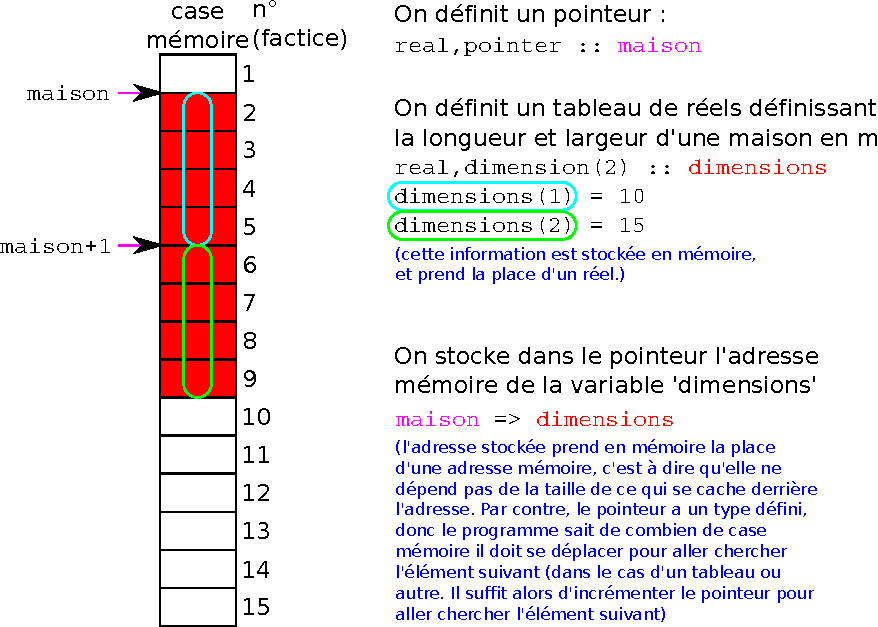
\includegraphics[width=0.65\linewidth]{figure/pointeurs.pdf}
\caption{Représentation schématique du fonctionnement d'un pointeur avec représentation de la mémoire. Les numéros pour les cases mémoires ne représentent pas la réalité, c'est juste pour montrer comment on fait référence à une case mémoire. L'idée est de montrer qu'en manipulant des adresses au lieu de manipuler les contenus, on peut faire des choses beaucoup plus puissantes.}
\end{figure}

%TODO lire des trucs sur les pointeurs, les types dérivés et les procédures récursives.

\end{document}